% -*- mode: noweb; noweb-default-code-mode: R-mode; -*-









\graphicspath{ {analysis/} }

\chapter{Analysis}
\label{cha:analysis}

% , eval=TRUE>>=



% latex table generated in R 2.13.0 by xtable 1.5-6 package
% Wed Jun 15 14:34:21 2011
\begin{table}[ht]
\begin{center}
{\small
\begin{tabular}{rrrrrrr}
  \hline
 & Agland2000 & NLCD & \pbox[c][][c]{3in}{Aggregated\\$A_{min}=0.5$} & \pbox[c][][c]{3in}{Aggregated\\$A_{min}=1.0$} & \pbox[c][][c]{3in}{No Mosaic\\$A_{min}=0.5$} & \smallskip\pbox[c][][c]{3in}{No Mosaic\\$A_{min}=1.0$} \\ 
  \noalign{\smallskip} \hline
crop & 446.5 & 310.8 & 378.9 & 369.6 & 495.4 & 488.1 \\ 
  open & 557.1 & 429.6 & 516.9 & 545.8 & 538.7 & 561.9 \\ 
  barren & 0.0 & 24.5 & 32.8 & 28.9 & 32.8 & 28.9 \\ 
  forest & 0.0 & 513.2 & 344.7 & 353.6 & 410.8 & 429.9 \\ 
  mosaic & 0.0 & 0.0 & 232.9 & 237.0 & 0.0 & 0.0 \\ 
  shrub & 0.0 & 420.1 & 358.7 & 341.8 & 387.2 & 368.0 \\ 
  urban & 0.0 & 102.8 & 27.3 & 29.8 & 27.3 & 29.8 \\ 
  water & 0.0 & 96.5 & 74.3 & 75.0 & 74.3 & 75.0 \\ 
  wetland & 0.0 & 95.0 & 26.0 & 11.0 & 26.0 & 11.0 \\ 
  total & 1003.7 & 1992.5 & 1992.5 & 1992.5 & 1992.5 & 1992.5 \\ 
   \noalign{\smallskip} \hline
\end{tabular}
}
\caption{Total Acreages by Map and Cover}
\label{tab:areas}
\end{center}
\end{table}
\begin{figure}[hpt] 
\begin{center} 


\includegraphics{fig_areas}
\end{center} 
\caption{Total Acreages by Map and Cover}
\label{fig:areas} 
\end{figure} 


After decomposing the mosaic class The MLCT indicates
495.4Ma (200.5Mha) of cropland for
$A_{min}=0.5$ and 488.1Ma (197.5Mha) for
$A_{min}=1.0$ in the cUSA in 2001. 

Pasture indicated by Aglands2000 appears to be a broader
classification than that of the NLCD's pasture class because much of
the grazing land east of the Mississippi river counted in the
Aglands2000 pasture map is absent in the NLCD pasture class.

Aglands2000 indicates roughly
Ma (Mha) of cropland.  The
inability of the MLCT data set to resolve rural transportation
networks, minor settlements, and small water or wetland features is a
major contribution to the surplus of cropland acreage indicated by the
MLCT.  Due to its greater resolution, ~30m vs. ~500m, the NLCD is
better suited at discerning developed areas in rural landscapes
ranging from rural roads to farmsteads to small communities that do
not show up in the MLCT data. There is a total area of roughly 74 Ma
(30 Mha) of development remaining after subtracting the MLCT urban
class from all developed classes in the NLCD where the NLCD shows
greater development after they have both been aggregated to the
5-arcmin grid. Applying this area as an offset to the cropland area in
Aglands2000 brings us closer to the expected acreage under cultivation
in 2001, although this assumes that all of that development intersects
with MLCT cropland area.


The purpose for processing the MLCT for two values of $A_{min}$ as
described in the previous chapter is to evaluate whether or not
information from the secondary cover type contributes positively to
the accuracy of the data set we seek to synthesize.  The primary
objective of this synthesis is to achieve accuracy in cropland
distribution.  Because the cropland layer in the Agland2000 data set
is derived from county-level production census statistics we adopt
this as the ground truth and will endeavor to adjust our product
accordingly.  Although MLCT overstates cropland acreage for both
$A_{min}=0.5$ and $A_min=1.0$ the discrimination among the two is made
by the distribution of errors rather than the aggregate error.

\missingfigure{error map for ``nomos'' vs. Agland2000 crop}

These maps show the cell-by-cell differences between the MLCT-derived
data set that we have calculated after mosaic decomposition and the
Agland2000 cropland map.  TO summarize and compare these errors we
calculate the root of the mean squared error (RMSE) given by:

$$
\operatorname{RMSE}=\sqrt{\frac{\sum_{i=1}^{n}(\hat\theta_i-\theta_i )^2}{n}}
$$

where $\hat\theta_i$ are the predictions derived from the respective
MLCT derivations and $\theta_i$ are the observations taken from the
Agland2000 data set.



\begin{figure}[hpt]
  \begin{center} 


\includegraphics{fig_scatPlot1}
  \end{center} 
  \caption{Scatter plot of MLCT crop ($A_{min}=1.0$, no mosaic) versus Agland2000 cropland}
  \label{fig:scatplot1} 
\end{figure} 

\begin{figure}[hpt]
  \begin{center} 



\includegraphics{fig_scatPlot05}
  \end{center} 
  \caption{Scatter plot of MLCT crop ($A_{min}=0.5$, no mosaic) versus Agland2000 cropland}
  \label{fig:scatplot05} 
\end{figure} 

% latex table generated in R 2.13.0 by xtable 1.5-6 package
% Wed Jun 15 14:34:43 2011
\begin{table}[ht]
\begin{center}
\begin{tabular}{rr}
  \hline
$A_{min}$ & RMSE \\ 
  \hline
0.5 & 0.165 \\ 
  1.0 & 0.180 \\ 
   \hline
\end{tabular}
\caption{RMSE, MLCT vs. Agland2000 crop}
\label{tab:rmse}
\end{center}
\end{table}
The results on Table \ref{tab:rmse} indicate that $A_{min}=0.5$ is
more representative of the distribution of cropland because although
the total area indicated is higher there is less error on a
cell-by-cell basis indicating that it does a better job of
representing the spatial distribution than $A_{min}=1.0$.  Later when
we recalculate the cell proportions by accepting the values for
cropland area from Agland2000 as truth we can expect minimal
distortion in reconciling its landscape with that given by MLCT.  From
this point forward we will consider only the statistics derived from
setting $A_{min}=0.5$ for the aggregation of the MLCT data due to this
improved fit with Agland2000 cropland and its full consideration of
all information imparted by the MLCT data.


\section{NLCD Offsets}
\label{sec:nlcd_offsets}


From Table \ref{tab:areas} it is apparent that the MLCT results are
negatively biased in the areas assigned to water, wetland, and urban
features relative to the NLCD.  It is clear from visual inspection
that features of these classes tend to have smaller characteristic
dimensions which causes them to be overlooked in the the MLCT data due
to its resolution.  The most obvious example are the rural
transportation networks in areas delineated by the Public Land Survey
System (PLSS) where roads have been laid out on a generally regular
grid of square miles.  In the PEEL classification this infrastructure
is included in the urban class as another form of developed land.  It
is important to represent wetlands and water features in our input to
the PEEL model because these areas have high likliehoods of being set
aside for conservation purposes, which would be represented as a
constraint on land conversion in the model.

To merge this information from the NLCD we begin by simply accepting
the areas for water, wetland, and urban classes in the reclassified,
5$'$-aggregated version of NLCD that we have computed as truth and
calculate offsets for those classes versus our 5$'$ MLCT data by
straight subtraction.  The other classes are then adjusted so that
they are present in proportion to each other as indicated by MLCT but
in the area remaining after accepting the water, wetland, and urban
areas from NLCD.  The additive offsets needed to achieve this balance
and account for the entire area of the cell are calculated so that the
effects of this process on all classes may be considered on a common
basis.


\begin{figure}[hpt]
  \begin{center} 


\includegraphics{fig_offsets1}
  \end{center} 
  \caption{NLCD offsets}
  \label{fig:offsets1} 
\end{figure} 

\begin{figure}[hpt]
  \begin{center} 


\includegraphics{fig_offsets2}
  \end{center} 
  \caption{NLCD offsets (cont.)}
  \label{fig:offsets2} 
\end{figure} 


\autoref{fig:offsets1} and \autoref{fig:offsets2} show the spatial distributions of the offsets calculated based on our assumptions about the water, wetland, and urban classes in the NLCD.




\begin{figure}[hpt]
  \begin{center} 
    \includegraphics{fig_corOffsets}
  \end{center} 
  \caption{Covariance matrix of NLCD offsets}
  \label{fig:corOffsets} 
\end{figure} 

The resulting offsets are added to the aggregated fractions calculated
from the MLCT with $A_{min}=0.5$.  








Following these algebraic acrobatics it seems prudent to check our
accounting with some simple arithmetic.  Working backwards from the
final result of adding NLCD-derived offsets to the raster stack
derived from the MLCT with $A_{min}=0.5$ and decomposing the remaining
mosaic fractions into their constituent cover types, subtracting the
deltas that came from the mosaic decomposition, subtracting offsets
calculated from the NLCD, and subtracting the aggregated MLCT data
from the previous chapter 
\todo{hyperlink to section where MLCT was aggregated} 
should produce zeroes everywhere, plus or minus the noise of floating
point math.




\begin{Schunk}
\begin{Soutput}
class       : RasterBrick 
dimensions  : 298, 695, 9  (nrow, ncol, nlayers)
resolution  : 0.08333333, 0.08333333  (x, y)
extent      : -124.8333, -66.91667, 24.5, 49.33333  (xmin, xmax, ymin, ymax)
projection  : +proj=longlat +ellps=WGS84 +datum=WGS84 +no_defs +towgs84=0,0,0 
values      : in memory
min values  : -2.8e-17 -1.1e-16 -1.1e-16 -1.1e-16 -5.6e-17 -1.1e-16 -5.6e-17 -1.1e-16 -1.1e-16 
max values  : 2.8e-17 1.1e-16 1.1e-16 1.1e-16 5.6e-17 1.1e-16 5.6e-17 1.1e-16 1.1e-16 
\end{Soutput}
\end{Schunk}

% latex table generated in R 2.13.0 by xtable 1.5-6 package
% Wed Jun 15 14:38:14 2011
\begin{table}[ht]
\begin{center}
\begin{tabular}{rrrr}
  \hline
 & class & min & max \\ 
  \hline
water & 0 & -2.78E-17 & 2.78E-17 \\ 
  forest & 1 & -1.11E-16 & 1.11E-16 \\ 
  shrub & 2 & -1.11E-16 & 1.11E-16 \\ 
  open & 3 & -1.11E-16 & 1.11E-16 \\ 
  wetland & 4 & -5.55E-17 & 5.55E-17 \\ 
  crop & 5 & -1.11E-16 & 1.11E-16 \\ 
  urban & 6 & -5.55E-17 & 5.55E-17 \\ 
  mosaic & 7 & -1.11E-16 & 1.11E-16 \\ 
  barren & 8 & -1.11E-16 & 1.11E-16 \\ 
   \hline
\end{tabular}
\caption{Balance of adjustment fractions and original MLCT aggregation}
\label{tab:restack_check}
\end{center}
\end{table}
To assess whether the process of adding in the NLCD offsets has
improved overall cropland accuracy we can perform the same error
calculation from above and extend Table~\ref{tab:rmse} with the new
result, giving us Table~\ref{tab:rmse2}.

% latex table generated in R 2.13.0 by xtable 1.5-6 package
% Wed Jun 15 14:38:20 2011
\begin{table}[ht]
\begin{center}
\begin{tabular}{lrrr}
  \hline
offset & $A_{min}$ & $RMSE_{crop}$ & $RMSE_{open}$ \\ 
  \hline
TRUE & 0.5 & 0.151 & 0.236 \\ 
  FALSE & 0.5 & 0.165 & 0.242 \\ 
  FALSE & 1.0 & 0.180 & 0.267 \\ 
   \hline
\end{tabular}
\caption{RMSE, MLCT vs. Agland2000 crop with NLCD offsets}
\label{tab:rmse2}
\end{center}
\end{table}
\todo[caption=Should the RMSE tables be rearranged?]{Would it make
  more sense to have the row order and independent variables (first
  three) reversed in Table \ref{tab:rmse} and \ref{tab:rmse2}?}

Seeing that this modifcation to the data set has improved our overall
accuracy of the distribution of croplands the next step is to examine
the total areas for all classes compared with the input data sets.  


% latex table generated in R 2.13.0 by xtable 1.5-6 package
% Wed Jun 15 14:38:20 2011
\begin{table}[ht]
\begin{center}
{\small
\begin{tabular}{rrrrrrrr}
  \hline
 & Agland2000 & NLCD & MLCT & \pbox[c][][c]{3in}{MLCT\\No Mosaic} & \pbox[c][][c]{3in}{NLCD\\Offsets} & \pbox[c][][c]{3in}{MLCT\\Adjusted} & \pbox[c][][c]{3in}{\smallskip{}MLCT\\Adjusted\\No Mosaic} \\ 
  \noalign{\smallskip} \hline
water & 0.0 & 96.5 & 74.3 & 74.3 & 22.3 & 96.5 & 96.5 \\ 
  forest & 0.0 & 513.2 & 344.7 & 410.8 & -44.7 & 300.1 & 355.7 \\ 
  shrub & 0.0 & 420.1 & 358.7 & 387.2 & -23.8 & 334.9 & 358.0 \\ 
  open & 557.1 & 429.6 & 516.9 & 538.7 & -21.0 & 495.9 & 514.9 \\ 
  wetland & 0.0 & 95.0 & 26.0 & 26.0 & 69.0 & 95.0 & 95.0 \\ 
  crop & 446.5 & 310.8 & 378.9 & 495.4 & -39.0 & 339.9 & 437.6 \\ 
  urban & 0.0 & 102.8 & 27.3 & 27.3 & 75.4 & 102.8 & 102.8 \\ 
  mosaic & 0.0 & 0.0 & 232.9 & 0.0 & -37.4 & 195.5 & 0.0 \\ 
  barren & 0.0 & 24.5 & 32.8 & 32.8 & -0.9 & 31.9 & 31.9 \\ 
  (all) & 1003.7 & 1992.5 & 1992.5 & 1992.5 & -0.0 & 1992.5 & 1992.5 \\ 
   \noalign{\smallskip} \hline
\end{tabular}
}
\caption{Effect of NLCD offsets on total acreages, $A_{min}=0.5$}
\label{tab:areas2}
\end{center}
\end{table}
\begin{figure}[hpt]
  \centering

 

  \includegraphics{fig_offsets}
  \caption{Total offsets calculated from NLCD}
  \label{fig:offsets}
\end{figure}


\begin{figure}[hpt]
  \centering


  \includegraphics{fig_areasAdj}
  \caption{Area totals after NLCD adjustment}
  \label{fig:areasAdj}
\end{figure}

\begin{figure}[hpt] 
  \begin{center} 


    \includegraphics{fig_scatPlotAdj}
  \end{center} 
  \caption{Scatter plot of MLCT adjusted crop versus Agland2000 cropland}
  \label{fig:scatPlotAdj} 
\end{figure} 





\begin{figure}[hpt] 
\begin{center} 


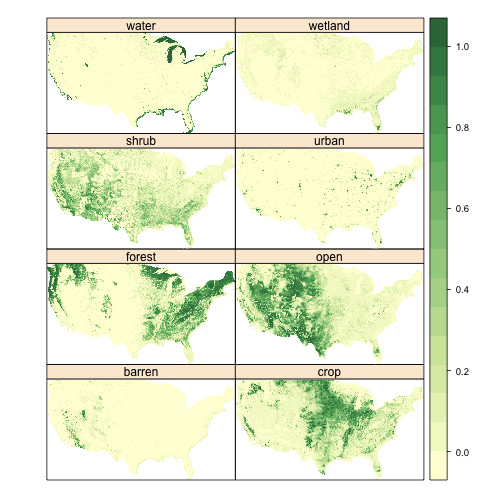
\includegraphics{fig_agc}
\end{center} 
\caption{Agland Complete cover maps} 
\label{fig:agc} 
\end{figure} 



blah blah blah

% latex table generated in R 2.13.0 by xtable 1.5-6 package
% Wed Jun 15 14:39:37 2011
\begin{table}[ht]
\begin{center}
\begin{tabular}{llrrr}
  \hline
agland & offset & $A_{min}$ & $RMSE_{crop}$ & $RMSE_{open}$ \\ 
  \hline
TRUE & TRUE & 0.5 & 0.017 & 0.208 \\ 
  FALSE & TRUE & 0.5 & 0.151 & 0.236 \\ 
  FALSE & FALSE & 0.5 & 0.165 & 0.242 \\ 
  FALSE & FALSE & 1.0 & 0.180 & 0.267 \\ 
   \hline
\end{tabular}
\caption{RMSE of Agland Complete vs. Agland2000}
\label{tab:rmse3}
\end{center}
\end{table}
\begin{figure}[hpt] 
  \begin{center} 


    \includegraphics{fig_scatPlotAgc}
  \end{center} 
  \caption{Scatter plot of MLCT adjusted crop versus Agland2000 cropland}
  \label{fig:scatPlotAgc} 
\end{figure} 

% latex table generated in R 2.13.0 by xtable 1.5-6 package
% Wed Jun 15 14:39:50 2011
\begin{table}[ht]
\begin{center}
{\small
\begin{tabular}{rrrrrr}
  \hline
 & Agland2000 & NLCD & \pbox[c][][c]{3in}{MLCT\\No Mosaic} & \pbox[c][][c]{3in}{\smallskip{}MLCT\\Adjusted\\No Mosaic} & AgC \\ 
  \noalign{\smallskip} \hline
water & 0.0 & 96.5 & 74.3 & 96.5 & 96.6 \\ 
  forest & 0.0 & 513.2 & 410.8 & 355.7 & 380.9 \\ 
  shrub & 0.0 & 420.1 & 387.2 & 358.0 & 362.8 \\ 
  open & 557.1 & 429.6 & 538.7 & 514.9 & 479.1 \\ 
  wetland & 0.0 & 95.0 & 26.0 & 95.0 & 95.0 \\ 
  crop & 446.5 & 310.8 & 495.4 & 437.6 & 443.7 \\ 
  urban & 0.0 & 102.8 & 27.3 & 102.8 & 102.8 \\ 
  mosaic & 0.0 & 0.0 & 0.0 & 0.0 & 0.0 \\ 
  barren & 0.0 & 24.5 & 32.8 & 31.9 & 31.7 \\ 
  (all) & 1003.7 & 1992.5 & 1992.5 & 1992.5 & 1992.5 \\ 
   \noalign{\smallskip} \hline
\end{tabular}
}
\caption{Agland Complete (AgC) acreages, $A_{min}=0.5$}
\label{tab:areas3}
\end{center}
\end{table}

\begin{figure}[hpt] 
  \begin{center} 


    \includegraphics{fig_agcThemeMap}
  \end{center} 
  \caption{Thematic map of conflicts between NLCD offsets and Agland2000}
  \label{fig:agcThemeMap} 
\end{figure} 





\begin{figure}[hpt] 
  \begin{center} 

    \includegraphics{fig_cropSubClassesMap}
  \end{center} 
  \caption{Normalized fractions for crop sub-classes}
  \label{fig:cropSubClassesMap} 
\end{figure} 


We could assume that forage crops come from open class but we don't
know enough about the confusion between Aglands2000 pasture and the
open class in the first place.  The focus here is field crops so that
is the only class that we are attempting to disaggregate for now.
Tree and shrub crops could be taken from the corresponding cover
types, but assuming that they are caught up in that classification is
a blind leap and their areas are small.  On the other hand, their
economic impact may be disproportionate to their areas by virute of
price, but this will have to be studied more carefully.

Double-cropping is ignored for now by normalizing the crop fractions
by the sum of all crops, which can exceed unity in instances of
intense double-cropping.  The predominant double-cropping system in
the cUSA to our knowledge is soy followed by winter wheat, but there
may be others.  In areas where soy and wheat are double-cropped their
areas will be underestimated in this data set relative to that given
in the 175Crops2000 data set, subsequent to the NLCD offset
adjustment.  This issues also bears further study.



%%% Local Variables: 
%%% mode: latex
%%% TeX-master: "thesis"
%%% End: 

